\documentclass{article}
\usepackage[margin=1cm,bottom=1.5cm]{geometry}
\usepackage{tikz} 
\usetikzlibrary{shapes.geometric, arrows, positioning}

\begin{document}

\centering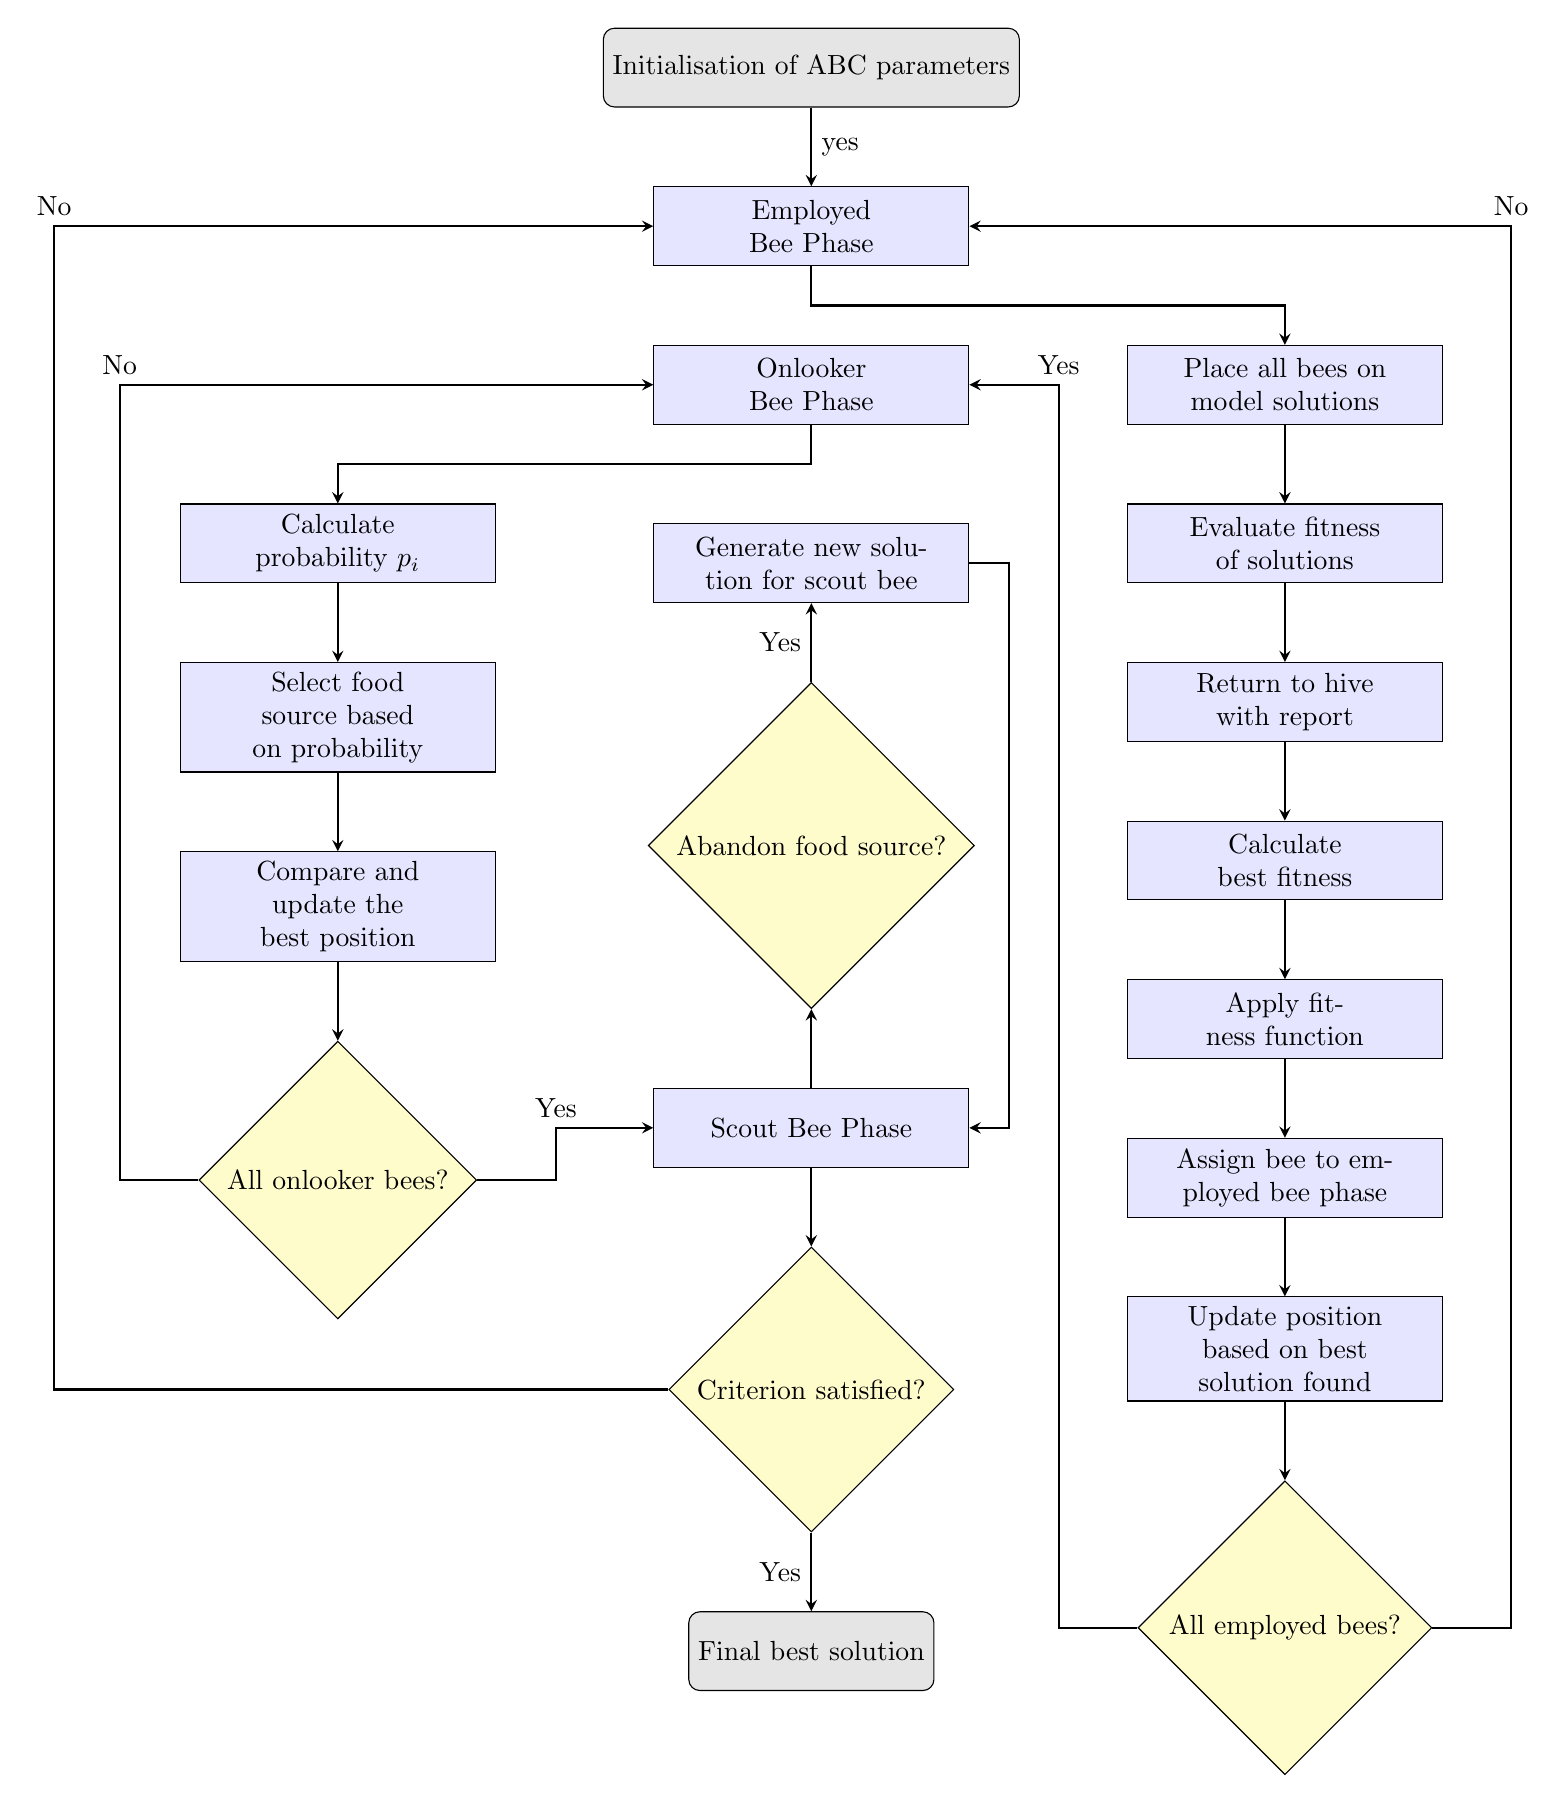
\begin{tikzpicture}[
node distance=1cm and 2cm,
% Define block styles 
startstop/.style = {rectangle, rounded corners, minimum width=3cm, minimum height=1cm, text centered, draw=black, fill=gray!20},
process/.style = {rectangle, minimum width=4cm, minimum height=1cm, text centered, draw=black, fill=blue!10,text width=3cm},
decision/.style = {diamond, minimum width=3.5cm, minimum height=1cm, text centered, draw=black, fill=yellow!20},
arrow/.style = {thick,->,>=stealth}
]

% Nodes
\node (start) [startstop] {Initialisation of ABC parameters};
\node (employedBee) [process, below=of start] {Employed Bee Phase};

% Steps within Employed Bee Phase
\node (placeBee) [process, below right=of employedBee] {Place all bees on model solutions};
\node (evaluate) [process, below=of placeBee] {Evaluate fitness of solutions};
\node (returnBee) [process, below=of evaluate] {Return to hive with report};
\node (bestFit) [process, below=of returnBee] {Calculate best fitness};
\node (applyFitness) [process, below=of bestFit] {Apply fitness function};
\node (assignBee) [process, below=of applyFitness] {Assign bee to employed bee phase};
\node (update) [process, below=of assignBee] {Update position based on best solution found};
\node (employedDecision) [decision, below=of update] {All employed bees?};

% Onlooker Bee Phase
\node (onlookerBee) [process, below=of employedBee] {Onlooker Bee Phase};

% Steps within Onlooker Bee Phase
\node (calcProb) [process, below left=of onlookerBee] {Calculate probability \( p_i \)};
\node (selectSource) [process, below=of calcProb] {Select food source based on probability};
\node (compareBest) [process, below=of selectSource] {Compare and update the best position};
\node (onlookerDecision) [decision, below=of compareBest] {All onlooker bees?};

% Scout Bee Phase
\node (scoutBee) [process, below right=of compareBest,yshift=-0.6cm] {Scout Bee Phase};
\node (abandon) [decision, above=of scoutBee] {Abandon food source?};
\node (generateNew) [process, above=of abandon] {Generate new solution for scout bee};

% Stopping Criteria
\node (stopping) [decision, below=of scoutBee] {Criterion satisfied?};
\node (final) [startstop, below=of stopping] {Final best solution};

% Arrows
\draw [arrow] (start) -- node[auto] {yes} (employedBee);
\draw [arrow] (employedBee.south) --++(0,-0.5) -| (placeBee);
\draw [arrow] (placeBee) -- (evaluate);
\draw [arrow] (evaluate) -- (returnBee);
\draw [arrow] (returnBee) -- (bestFit);
\draw [arrow] (bestFit) -- (applyFitness);
\draw [arrow] (applyFitness) -- (assignBee);
\draw [arrow] (assignBee) -- (update);
\draw [arrow] (update) -- (employedDecision);
\draw [arrow] (employedDecision.east) -- ++(1,0) |- node[anchor=south] {No} (employedBee);
\draw [arrow] (employedDecision.west) -- ++(-1,0) |-node[anchor=south] {Yes} (onlookerBee);

\draw [arrow] (onlookerBee.south) -- ++(0,-0.5) -| (calcProb);
\draw [arrow] (calcProb) -- (selectSource);
\draw [arrow] (selectSource) -- (compareBest);
\draw [arrow] (compareBest) -- (onlookerDecision);
\draw [arrow] (onlookerDecision.east) -- ++(1,0) |- node[anchor=south] {Yes} (scoutBee);
\draw [arrow] (onlookerDecision.west) -- ++(-1,0) |- node[anchor=south] {No} (onlookerBee);

\draw [arrow] (scoutBee) -- (stopping);
\draw [arrow] (stopping) -- node[anchor=east] {Yes} (final);
\draw [arrow] (stopping.west) -- ++(-7.8,0) |- node[anchor=south] {No} (employedBee.west);

\draw [arrow] (scoutBee) -- (abandon);
\draw [arrow] (abandon) -- node[anchor=east] {Yes} (generateNew);
\draw [arrow] (generateNew.east) -- ++ (0.5,0) |- (scoutBee.east);
\end{tikzpicture}

\end{document}
